\documentclass[a4paper, 11pt, final, garamond]{book}
\usepackage{cours-preambule}

\raggedbottom

\makeatletter
\renewcommand{\@chapapp}{Travaux pratiques -- TP}
\makeatother

\let\SavedIndent\indent
\protected\def\indent{%
  \begingroup
    \parindent=\the\parindent
    \SavedIndent
  \endgroup
}
\setlength{\parindent}{0pt}

\begin{document}
\setcounter{chapter}{6}

\chapter{Circuits du premier ordre en r\'egime transitoire}
\section{Objectifs}

\begin{itemize}
    \item Réaliser des montages simples d'électricité.
    \item Déterminer expérimentalement un temps de relaxation.
    \item Observer les différents paramètres qui influent sur un régime
        transitoire.
    \item Observer les différents régimes du second ordre.
    \item Découvrir quelques fonctions nouvelles de l'oscilloscope et du GBF.
    \item Mettre en œuvre la méthode  d'Euler à l'aide de Python pour simuler la
        réponse d'un système linéaire du premier ordre à une excitation
        quelconque.
\end{itemize}

\section{S'approprier}

\subsection{Règles de bonne pratique}

En pratique, on commence toujours par effectuer les branchements du circuit sans
insérer les appareils de mesure. Puis, on \textbf{relie toutes les masses entre
elles} afin d'éviter de fixer par erreur une autre masse dans le circuit. Ainsi,
un bon circuit aura une «~ligne de masse~» à laquelle seront reliés
obligatoirement tous les câbles noirs provenant des câbles coaxiaux-filaires
reliés à l'oscilloscope ou au GBF. Enfin, on place alors le fil rouge des câbles
de mesure aux endroits où on désire relever la tension. Vous serez d'ailleurs
également vigilant au choix de couleurs des fils, sinon on se perd rapidement…
Ces règles sont fondamentales et ne doivent pas être négligées si on veut que le
circuit fonctionne.

\subsection{Circuit intégrateur}

Un montage est considéré comme \textbf{intégrateur} (on le verra en cours dans
quelques semaines) si la tension de sortie (dans notre cas $u_{c}(t)$) est une
primitive, à une constante multiplicative $K$ près, de la tension d'entrée (dans
notre cas $e(t)$), soit encore

\[u_{c}(t) = K \int e(t) \dt\]

\subsection{Utilisation des oscilloscopes}

\subsubsection{Imprimer une courbe avec un oscilloscope Rigol}

\begin{enumerate}
    \item Allumer l'ordinateur et se connecter au réseau.
    \item Puis, programme, discipline, physique-chimie, physique, oscillo rigol.
    \item Tools, connect to oscillo, puis refresh.
    \item Passer en noir et blanc (B \& W) et enfin print.
\end{enumerate}

\subsubsection{Imprimer une courbe avec un oscilloscope Tektronix}

\begin{minipage}{0.49\linewidth}
    \begin{enumerate}
        \item Ouvrir Open Choice Desktop.
        \item Sélectionner instrument USB
        \item Afficher écran.
        \item Copier vers le presse-papier.
        \item Ouvrir paint et coller.
        \item Puis cliquer droit, inverser les couleurs.
    \end{enumerate}
\end{minipage}
\begin{minipage}{0.49\linewidth}
    \begin{enumerate}[start=6]
        \item Sélection rectangulaire, pour ne garder que les oscillogrammes et les
            réglages de l'oscilloscope.
        \item Copier~; Basculer dans libre-office ou word et Coller~;
        \item Faire une belle mise en page et mettre des titres et commentaires
            éventuels.
        \item Imprimer~!
    \end{enumerate}
\end{minipage}


\section{Analyser}

\begin{NCror}[width=\linewidth, halign=center]{Important}
    Cette partie est à faire chez vous (avec l'aide éventuelle du cours) avant
    la séance de TP.
\end{NCror}

\subsection{Étude théorique du régime transitoire du circuit RC}

\subsubsection{Charge et décharge du condensateur}

\begin{wrapfigure}[5]{r}{0.30\linewidth}
    \begin{center}
        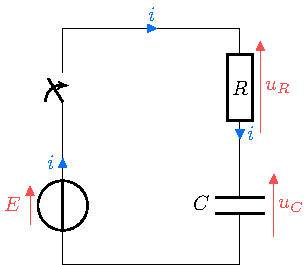
\includegraphics[width=\linewidth]{circ_rc-start}
    \end{center}
\end{wrapfigure}

On considère le montage ci-contre de constante de temps $\tau = RC$.

\begin{enumerate}
    \item Si $e(t)$ est une tension créneau de fréquence $f = \SI{1}{kHz}$,
        quelle valeur faut-il donner à $\tau$ pour visualiser de façon
        satisfaisante la totalité du régime transitoire~? Expliquer les raisons
        de votre choix. 
    \item Si $\tau$ est trop grand ou si $\tau$ est trop petit, que se
        passe-t-il~? 
    \item Si $R = \SI{1}{k\Omega}$, quelle valeur faut-il alors donner à $C$~? 
    \item On veut visualiser à l'oscilloscope simultanément $e(t)$ sur la voie 1
        et $u_{C}(t)$ sur la voie 2~; indiquer sur un schéma les connexions à
        réaliser.
\end{enumerate}

\subsubsection{Étude théorique du circuit intégrateur}

L'équation différentielle vérifiée par $u_{C}(t)$ est

\[\frac{\dd u_{C}(t)}{\dd t} + \frac{u_{C}(t)}{\tau} = \frac{e(t)}{\tau}\]

Supposons que à $t=0$, $e(t)$ passe de $0$ à $E$.

\begin{enumerate}[resume]
    \item Déterminer la solution de l'équation différentielle précédente dans
        le cas où $u_{C}(t=0) = 0$. En utilisant un développement limite du
        terme exponentiel, montrer que le montage est intégrateur (la sortie est
        une primitive de l'entrée).
\end{enumerate}

\medskip

\begin{instruc}[tikz={rotate=180, transform shape}]{Aide}
   Le développement limité de l'exponentiel s'écrit
   \[\text{e}^x \Sim_{x \to 0} 1+x + o(x)\]
\end{instruc}

\subsubsection{Circuit RC avec visualisation de $e(t)$ et $u_{R}(t)$}

On souhaite maintenant visualiser $e(t)$ sur la voie 1 et $u_{R}(t)$ sur la voie
2.

\begin{enumerate}[resume]
    \item Comment faut-il modifier le montage~? Sur votre feuille, faire le
        schéma du montage correspondant en indiquant les branchements de
        l'oscilloscope. 
    \item Écrire l'équation différentielle vérifiée par la variable $u_{R}(t)$
        et en donner la solution pour $e(t) = E$ et $u_{R}(t=0^-) = 0$.
        Attention, la tension n'est \textit{a priori} pas continue aux bornes de
        $R$…
\end{enumerate}

\subsection{Détermination numérique de la solution}

\subsubsection{Position du problème}

Comme vu dans la partie précédente, $u_{C}(t)$ est solution de l'équation
différentielle~:

\[\frac{\dd u_{C}(t)}{\dd t} + \frac{u_{C}(t)}{\tau} = \frac{e(t)}{\tau}\]

L'objectif de cette partie est de déterminer \textbf{numériquement} la solution
$u_{C}(t)$ de cette équation pour une entrée quelconque $e(t)$ pour laquelle il
n'existe pas toujours de solutions analytiques. Nous allons utiliser un schéma
numérique classique appelé Méthode d'Euler. En pratique, cette méthode est
relativement peu efficace (et des méthodes plus sophistiquées sont souvent mises
en place). Néanmoins la méthode d'Euler, très simple à comprendre et à mettre en
place, permet une première approche simple du problème.

\subsubsection{Méthode d'Euler~: mathématiquement}

Des théorèmes assurent que, sous des conditions raisonnables, il existe une
unique application $y$ de classe $C^1$ sur $[a,b]$ dont la valeur est imposée en
$a$ et qui vérifie une équation différentielle de la forme $y'(t)=f(t,y(t))$
pour tout $t \in [a,b]$. L'objet des \textit{schémas numériques} est d'obtenir
des approximations de cette solution.\bigbreak

En pratique, on tente d'approcher $y$ en un certain nombre de points répartis
sur l'intervalle $[a,b]$. Plus précisément, on veut calculer une approximation
$y_k$ des $y(t_k)$ avec $t_k=a+kh$ où $h=\dfrac{b-a}{n}$ est un pas qu'il
conviendra d'ajuster (on peut supposer que plus le pas est petit, meilleure sera
l'approximation). De façon simple, on peut écrire~:

\[y(t_{k+1})-y(t_k) =
    \int_{t_k}^{t_{k+1}}y'(u) \dd u =
    \int_{t_k}^{t_{k+1}} f(u,y(u)) \dd u \approx
h f(t_k,y(t_k))\]

On obtient alors la méthode d'Euler explicite~: les approximations sont
calculées de proche en proche via la formule suivante~:

$$y_{k+1}=y_k+hf(t_k,y_k)$$

On initialise bien entendu avec $y_0=y(a)$, qui sera la seule valeur «~exacte~»
calculée.

\begin{center}
    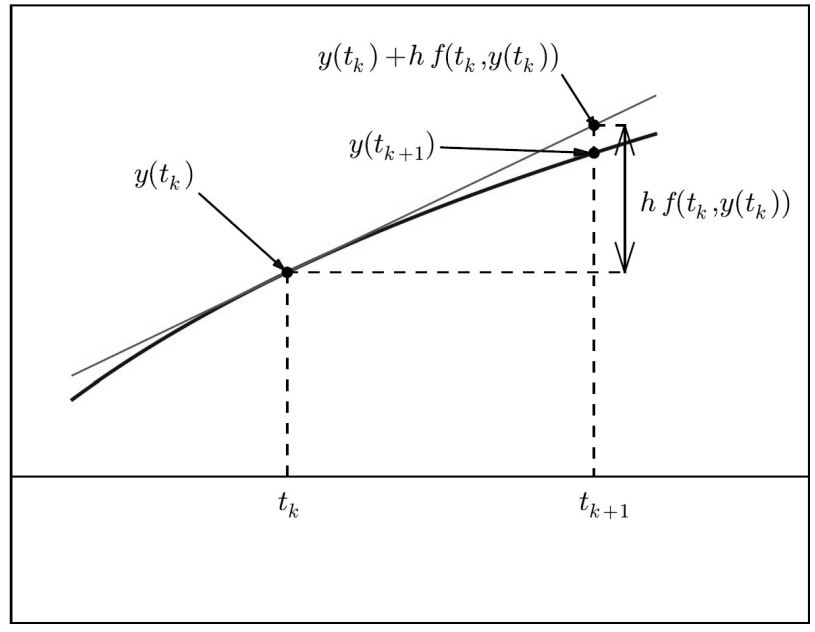
\includegraphics[scale=0.6]{euler}
\end{center}

\section{Réaliser et valider}

\subsection{Étude expérimentale du régime transitoire du circuit RC}

\subsubsection{Cas général~: charge et décharge du condensateur}

\begin{enumerate}
    \item Réaliser le montage RC proposé dans la partie Analyser.
    \item $e(t)$ est la tension créneau (alternance de tension nulle et de
        tension constante $E$) d'un générateur basses fréquences, réglé sur une
        fréquence de $\SI{1}{kHz}$.
    \item $R$ est une boîte de résistances variables~; Prendre $R =
        \SI{1}{k\Omega}$.
    \item $C$ est une boîte de capacités réglables~; Prendre la valeur calculée
        dans la partir analyse.
    \item Observer $e(t)$ et $u_{C}(t)$.
    \item Imprimer vos courbes en suivant le protocole proposé dans S'approprier
    \item Déterminer la constante de temps $\tau_{\rm exp}$. Expliquer votre
        démarche.
    \item Calculer \textbf{et commenter} l'écart relatif $\Delta$ par rapport à
        la valeur théorique~:
        \[\Delta = \frac{\abs{\tau_{\rm exp}-\tau_{\rm th}}}{\tau_{\rm th}}\]
    \item Étudier l'influence de $R$ et de $C$. Faire varier également la
        fréquence du signal périodique. Commenter vos observations. Il n'est pas
        demandé de refaire de nouvelles mesures. Une analyse qualitative est
        suffisante.
\end{enumerate}

\subsubsection{Cas particulier du circuit intégrateur}

Ne pas modifier le montage précédent, $e(t)$ est toujours une tension créneau.

\medskip

\begin{itemize}
    \item Choisir $\tau$ de l'ordre de $10 T$ en ajustant la valeur de $R$ et
        observer $e(t)$ et $u_{C}(t)$.
    \item Quelle est l'allure de $u_{C}(t)$~? $u_{C}(t)$ est-elle bien la
        primitive de $e(t)$ à une constante multiplicative près?
    \item Déterminer expérimentalement la pente de la courbe $u_{C}(t)$ en vous
        aidant des curseurs (\textbf{pour toute mesure avec le curseur, vérifier
            que la source du menu curseur correspond bien à la courbe sur
        laquelle vous faites des mesures}). Comparer à la valeur théorique.
\end{itemize}

\medskip

Conserver les valeurs de $\tau$ et $T$. Changer la tension créneau par une dent
de scie.

\medskip

\begin{itemize}
    \item Quelle est l'allure de $u_{C}(t)$~? Le circuit est-il à priori
        toujours intégrateur~?
    \item Quelle est l'expression mathématique (aucun calcul à effectuer) de la
        courbe $u_{C}(t)$~?
\end{itemize}

 \medskip

Conserver les valeurs de $\tau$ et $T$. Changer la tension créneau par une
tension sinusoïdale.

\medskip

\begin{itemize}
    \item Quelle est l'allure de $u_{C}(t)$~? Le circuit est-il toujours
        intégrateur~?
    \item Quelle est l'expression mathématique (aucun calcul à effectuer) de la
        courbe $u_{C}(t)$~?
\end{itemize}

\medskip

Augmenter $\tau$, quel inconvénient apparaît~? Commenter vos observations.

\subsubsection{Tension aux bornes de la résistance $u_R$}

Se placer dans les mêmes conditions que dans la partie IV.A.1 et observer à
l'oscilloscope $e(t)$ et $u_{R}(t)$. Imprimer les résultats. Commenter l'allure
de la courbe. Est-elle conforme à l'expression analytique attendue~?

\subsection{Étude numérique}

\subsubsection{Écriture du script}

Vous avez dans un premier temps besoin d'importer les bibliothèques Python
suivantes~:

\begin{python}
import matplotlib.pyplot as plt
import numpy as np
\end{python}

Compléter ensuite la fonction \texttt{euler(f, a, b, y0, n)} suivante qui, étant
données une fonction $f$, des valeurs de $a$ et $b$, un entier $n$ et une
condition initiale $y0$ calcule les valeurs approchées sur $[a,b]$ de la
solution de l'équation différentielle $y'(t)=f(t,y(t))$ avec la condition
initiale $y(a)=y0$. Cette fonction renverra le tableau des $n+1$ valeurs
approchées $y_k$ de $y$ aux temps $t_k=a+k \frac{b-a}{n}$, $k\in[\![0,n]\!]$.

\begin{python}
def euler(f, a, b, y0, n):
    h = (b-a) / n
    tab_y = [y0]
    y = y0
    t = a
    for i in range(n):
        y = # à compléter
        t = # à compléter
        tab_y.append(y)
    return tab_y
\end{python}

Il faut ensuite créer la fonction \texttt{f} ainsi que la fonction entrée
\texttt{e} pour plus de clarté. Vous compléterez la fonction \texttt{f} pour
qu'elle renvoie l'expression correspondant à l'équation différentielle que vous
cherchez à résoudre.

\begin{python}
def f(t, y, e):
    return # à compléter

# définitions des différentes entrées
def e(t): #entrée constante
    return 10 # np.sin(t)
\end{python}

L'exemple proposé ici est dans le cas d'une entrée constante d'amplitude $E =
10$. Vous pouvez alors changer la fonction \texttt{e(t)} si vous voulez explorer
les solutions pour d'autres formes d'entrée.

Enfin, il est possible de récupérer les valeurs $y$ de la solution par

\begin{python}
tau = 1
tps = np.linspace(0, 10, n+1) # vecteur temps entre t = 0 et t = 10
tab_y = euler(f, 0 , 10, 0, n) # tab_y est un vecteur des valeurs de y
\end{python}

\subsubsection{Test dans un cas analytique}

Tester votre fonction précédente avec une entrée constante $e(t) = E$ afin de
résoudre l'équation différentielle sur $u_{C}(t)$. Afficher sur un même
graphique la solution numérique et la solution analytique que vous déterminerez.
On pourra, par choix et pour fixer les idées, sans que cela porte à conséquence
prendre~:

\centers{$E = \SI{1}{V} \qquad \qquad \tau = \SI{1}{s} \qquad \qquad u_{C}(t=0) = 0$}

Vous afficherez également la fonction erreur au cours du temps, qui est la
différence entre votre solution numérique et la solution analytique. Quelle est
la sensibilité au pas de calcul~? Vous ferez plusieurs essais.

\subsubsection{Test dans un cas non analytique}

Lorsque la solution $u_{C}(t)$ peut être obtenue analytiquement, la solution
numérique n'a que peu d'intérêt. Elle prend en revanche tout son sens dans des
cas non analytique. Testez votre programme pour plusieurs entrées (en changeant
le contenu de la fonction \texttt{e(t)})~: sinusoïdale, rampe linéaire,
exponentielle… Afficher le résultat et les imprimer (tous sur une unique feuille
A4).

\end{document}
